\subsubsection{Class and Custom Labs}

\newline
Custom labs are created for specific uses, such as hosting a class or a research team working on a project.

\paragraph{Cloud Resources in Custom Labs}

The resources provided in custom labs are based on the anticipated needs of a given user group and often differ from those provided in OpenSARLab. Requests for changes to compute and storage resources must be approved by the owner of a custom lab. This is typically a professor, workshop host, or PI on a grant-funded project.

\paragraph{Custom Lab Access}

Access to all custom labs is determined by the owner of each lab. Professors, instructors, or PIs should provide instructions for accessing a custom lab. Access will require an \href{/opensciencelab-accounts}{OpenScienceLab account}.

Once a user's OpenScienceLab account has been given access to a lab, a lab access card will appear in the OpenScienceLab portal after signing in.

\begin{figure}[!htbp]
\centering
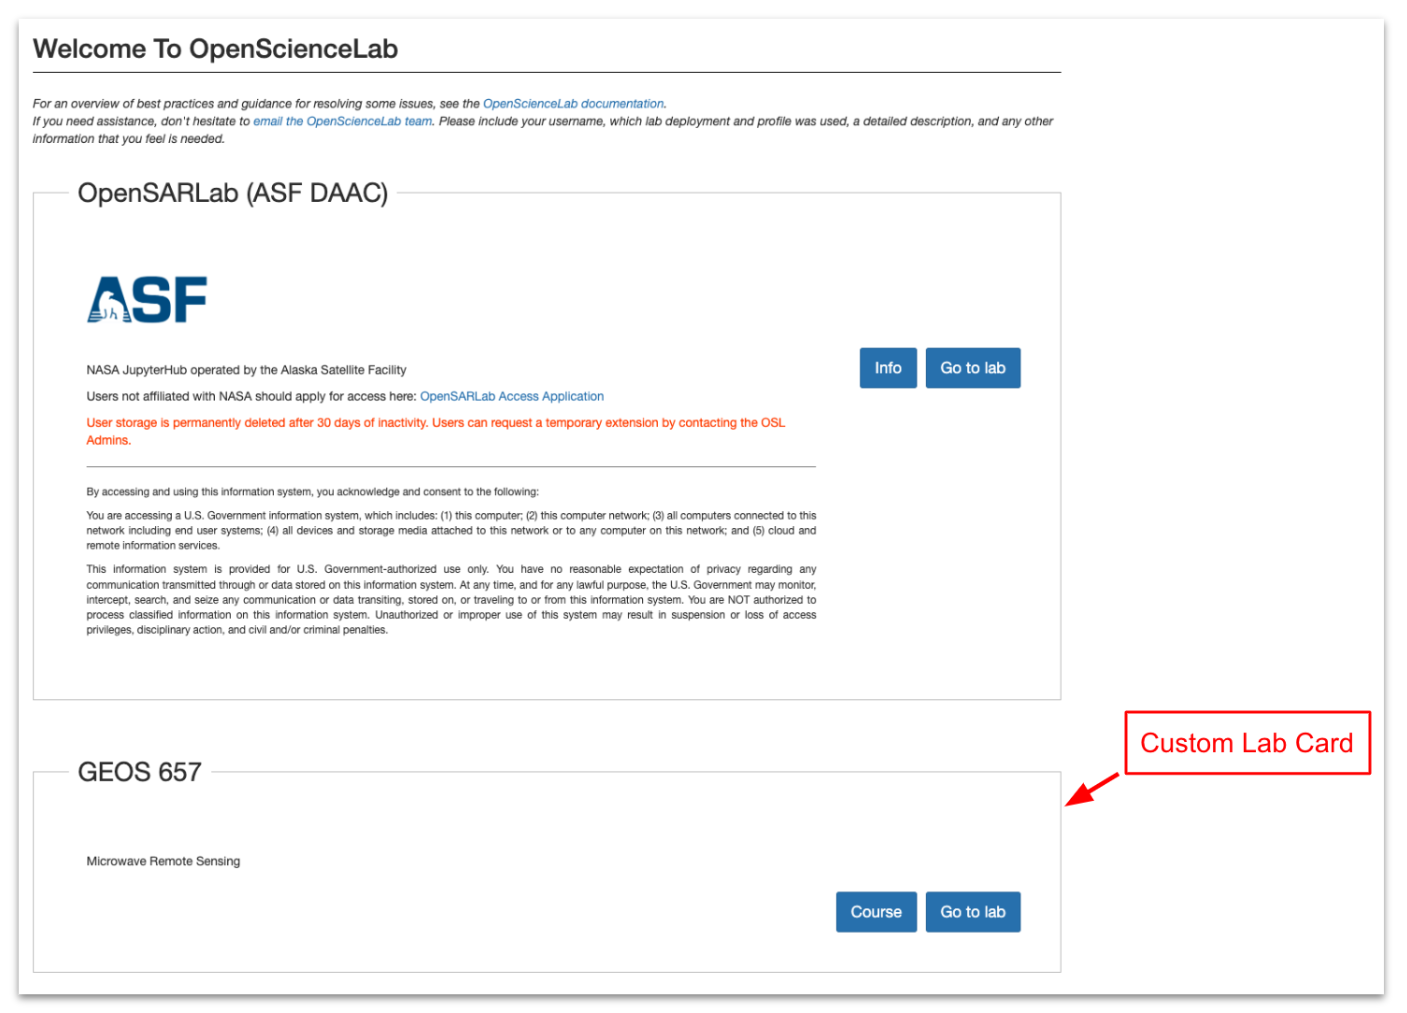
\includegraphics[width=0.7\linewidth]{files/opensciencelab_custo-3c1a84de52b386ba0c769f8989eeccea.png}
\caption*{OpenScienceLab with custom lab card}
\end{figure}